\chapter{\acl{fra}} \label{sec:haupt}
In diesem Kapitel soll auf die  Vorgehensweise und die Implementierung des in \ref{sec:konzept} vorgestellte \ac{fra} eingegangen werden. Die Schwerpunkte liegen hierbei bei der Beschreibung des generischen Plattformtreibers, den \ac{ioctl}s, der Kernel- bzw. Userspaceimplementierung sowie der Einbindung in die bestehende Software. Damit es der Umfang der Arbeit nicht übersteigt, wird nur die \acl{xbar} softwareseitig implementiert.

%Aktuelle Implementierung
%Theoretische Grundlagen o.ä.
%Umsetzung

\section{Generischer Plattformtreiber} \label{sec:plat}
Zunächst soll auf den Plattformtreiber eingegangen werden, der eine einwandfreie Kommunikation zwischen den Firmware Modulen im \ac{fpga} und dem Kernel gewährleisten soll.


Wie in dem Kapitel~\ref{sec:plat_t} bereits erläutert, werden für die grundlegende Funktionsweise eines Treiber verschiedene Funktionen benötigt. Zunächst soll auf die Registrierungs- bzw. Aufräumfunktion des Treibers eingegangen werden.\\


Beim Laden des Treibers werden verschiedene allgemeingültige Parameter gesetzt und zusätzlich Speicherplatz allokiert. 
\begin{lstfloat}
\begin{lstlisting}
struct afm_driver
{
	unsigned int major_id;

	uint8_t minor_list[AFM_MAX];
	spinlock_t minor_spinlock;
	struct class * class;
};
\end{lstlisting}
\captionof{code}{\label{code:afm_data}Struktur des Treibers}
\end{lstfloat}

Desweitern wird beim Laden als Erstes eine Klasse erstellt, der später die einzelnen Module zugeordnet werden. Diese Klasse wird in der, dem Treiber, zugehörigen Struktur \textit{afm\_driver} in der Variablen \textit{class} abgespeichert. 


Da die Majornummer den Treiber kennzeichnet (siehe Kapitel~\ref{sec:mmnum_t}) wird diese in der globalen Treiberstruktur als \textit{major\_id} gespeichert. Für die Minornummer wird in der Datenstruktur eine Liste \textit{minor\_list[AFM\_MAX]} und ein zugehöriges Spinlock \textit{minor\_spinlock} initialisiert. Über die Liste wird später eine freie Nummer ausgewählt, die bei jedem Module individuell ist und gleichzeitig wird dadurch die Anzahl der möglichen Module auf \textit{AFM\_MAX} begrenzt. Das Spinlock sorgt bei der Auswahl der Minornummer für einen konfliktfreien Vorgang, sodass keine Nummer doppelt vergeben werden kann. 


Am Ende der initialen Funktion wird der Plattformtreiber mit der \textit{platfrom\_driver} Struktur (siehe Codeausschnitt~\ref{code:platform_driver}) registriert. Damit werden die initiale Funktion zum Anlegen, aber auch die Funktion zum Deinitialisieren der Geräte übergeben.


Analog wird beim Freigeben des Treibers der allokierte Speicherplatz freigegeben, der Plattformtreiber abgemeldet und die erstellte Klasse zerstört.\\


Beim Anlegen einer Instanz vom Treiber wird die \textit{probe} Funktion des Plattformtreibers aufgerufen und zusätzlich wird der Modultyp und Name in einer \textit{arri\_fra\_mod\_config} Struktur zur Verfügung gestellt. In der initialen Funktion der Instanz wird diese Struktur genutzt um spezifische Einstellungen für jede einzelnes Gerät festgelegt und in einer entsprechenden Datenstruktur (siehe Codeausschnitt~\ref{code:afm_device}) gespeichert. 
%todo evtl tabelle zur erklärung!

%todo aussotieren
\begin{lstfloat}
\begin{lstlisting}
struct afm_device 
{
	struct arri_fra_mod_config *mod_config;
	
	struct class *class;
	struct cdev cdev;
	unsigned int minor_id;
	struct platform_device *pdev;
	struct resource *res;
	u8 __iomem *base;
	
	struct afm_file fdev[AFM_FILE_MAX];
	spinlock_t open_spinlock;
	%atomic_t use_count;
	
	#define AFM_NOLOGGING   ((uint32_t)0U)
	#define AFM_LOGGING     ((uint32_t)1U)
	uint32_t has_logging;
};
\end{lstlisting}
\captionof{code}{\label{code:afm_device}Auszug aus der Struktur einer Instanz}
\end{lstfloat}

Der einzige Übergabeparameter der Probefunktion ist die Struktur des \textit{platform\_device}, diese wird in dem Zeiger \textit{*pdev} gespeichert. Auch die, beim Laden des Treibers, angelegte Klasse wird ohne weitere Änderungen unter \textit{*class} abgelegt. 

Aus der Liste der Minornummern (siehe Codeausschnitt~\ref{code:afm_data}) wird nach dem Sperren des zugehörigen Spinlocks eine freie Nummer ausgewählt und als \textit{minor\_id} gespeichert, sowie in der Liste als verwendet gesetzt. Danach wird das Spinlock wieder freigegeben.

Anschließend wird mit Hilfe der Majornummer und der Minornummer ein Gerät erstellt und als \textit{cdev} gespeichert. 

%todo vorteile statischer speicher
Damit das Gerät der Devices auf eine bestimmte Anzahl limitiert ist, wird beim Initialisieren der Instanz ein Array der \textit{afm\_file} Struktur angelegt. Dadurch wird gleichzeitig der Speicherplatz statisch zur Kompilierzeit reserviert. Durch den Spinlock \textit{open\_spinlock} wird später dafür gesorgt, dass Kollisionen und Raceconditions vermieden werden.

%todo base/res

\section{Konzeptionierung der \acl{ioctl}s}\label{sec:ioctl}
%über ioctl zugriff auf das geöffnete Device
%Auf die ioctl eingehen und die Überlegungen hinter diesen
%hello, logging/unlogging?, get id, get reg, get reg bitmask, get reg block, set reg, set reg bitmask, set reg block, 
Damit der Zugriff und die Steuerung der Geräte, welche man über den generischen Treiber angelegt hat möglich ist, soll dieser Abschnitt auf die Konzeptionierung der \ac{ioctl}s eingehen.
Wie in Kapitel~\ref{sec:ioctl_t} erläutert werden diese benötigt, um zwischen Kernel und Userspace Daten auszutauschen. Da der Großteil der Software im Userspace läuft, aber der Treiber im Kernel, wird der hauptsächliche Zugriff auf die Geräte über \ac{ioctl}s geregelt. Die Überlegungen hinter den einzelnen \ac{ioctl}s werden im Folgenden näher erläutert.\\


Als Erstes ist eine Anmeldung der Anwendung bei dem Gerät notwendig. Um die Eindeutigkeit zu garantieren wird hier die \ac{pid} übergeben. Allerdings wird auch der Prozessname benötigt, damit eine schnelle Nachvollziehbarkeit bei der Fehlersuche auf der Kamera vorhanden ist.
%Wie in Kapitel~\ref{sec:konzept} erläutert, soll die Unterscheidung zwischen Standardapplikation und Debugtool möglich sein. Aus diesem Grund wird bei der Anmeldung zusätzlich zur \ac{pid} und dem Prozessnamen auch der Typ der Applikation übergeben. 
%todo satz hier oder wo anders?
Ohne die Ausführung von \textit{ARRI\_FRA\_MOD\_HELLO} bleibt der weitere Zugriff auf das Gerät über \ac{ioctl}s verwehrt, da die Anmeldung notwendig ist um im laufenden Betrieb eine Analyse vorzunehmen.\\

Die Protokollierung der Zugriffe auf ein Gerät ist ein notwendiger Bestandteil. Dadurch soll, vor allem im Fehlerfall, die Suche erleichtert werden. Aufgrund der Zugriffe durch verschiedene Prozesse besteht ohne Protokollierung kein einheitlicher Überblick über die Zugriffe.
In dem Zusammenhang werden zwei \ac{ioctl}s angelegt. Dabei ist \textit{ARRI\_FRA\_MOD\_LOGGING} zum Aktivieren der Nachrichten zuständig und analog wird diese durch \textit{ARRI\_FRA\_MOD\_NOLOGGING} deaktiviert. \\

Beim Anlegen des Geräts werden der Gerätetyp und der Name abgelegt. Im Userspace besteht die Notwendigkeit auf diese Informationen nach dem Öffnen des Geräts zuzugreifen. Dafür wird ein eigenes \ac{ioctl} benötigt, welches lediglich den Typ und Namen aus der Instanzstruktur (siehe Codebeispiel~\ref{code:afm_device}) zurück gibt.\\

Die essenziellen Funktionen des Treibers sind das Setzen bzw. Auslesen von Register. Basierend auf den, in der aktuellen Implementierung genutzten Funktionen und den entsprechenden Registerzugriffen, gibt es bis zu drei verschiedene Arten. Jede soll durch ein eigenes \ac{ioctl} abgebildet werden, da so die spätere Verwendung vereinfacht wird.  

%todo namen der ioctls einfügen -> tabelle erstellen
Die Größe eines Registers ist auf 4 Byte normiert. Damit werden zum einfachen Setzen eines Registers lediglich zwei Parameter benötigt. Zum Einen die Stelle des Registers im Gerät (auch Registernummer) und zum anderen der Inhalt. 
Allerdings besteht auch die Notwendigkeit einzelne Bits oder mehrere hintereinander liegende Register über einen Aufruf zu setzen. Für beide Sonderfälle gibt es ein gesondertes \ac{ioctl}. Zum Setzen von einzelnen Bits wird zusätzlich zu den beiden oben genannten Parametern noch eine Bitmaske übergeben. Mithilfe der Bitmaske werden im Register erst die entsprechenden Bits gelöscht und danach die übergebenen Bits gesetzt. Dadurch ist es nicht mehr notwendig erst das entsprechende Register auszulesen, anschließend zu verändern und dann in das gleiche Register zu setzen. So werden überflüssige  \ac{ioctl} und Registerzugriffe dezimiert.
Der zweite Sonderfall benötigt andere Übergabeparameter als das einfache Setzen. Zusätzlich zu der Registernummer wird hier eine Registeranzahl gebraucht. Des Weiteren muss der Inhalt für die Register in einem Array mit der Größe der Anzahl übergeben werden. Damit kann dann der Reihe nach jedes Register einzeln mit dem entsprechenden Inhalt beschrieben werden.


Das Auslesen der Register erfolgt nahezu analog zu dem Setzen. Der Parameter für den Registerinhalt wird hier allerdings über das \ac{ioctl} gefüllt und dann zurück in den Userspace übergeben. 
Register über eine Bitmaske auszulesen würde keine weiteren Vorteile gegenüber den Auslesen des ganzen Registers bieten. Aus diesem Grund wird es nicht implementiert.  
Damit man einen ganzen Block an Registern zurück lesen kann, muss durch das Übergeben eines Arrays mit der richtigen Größe des Speicherbereich zu Verfügung gestellt werden.\\

Dadurch sind die wichtigsten \ac{ioctl}s erläutert, die notwendig sind um die Grundfunktionen des Geräte abzudecken und zusätzlich eine triviale Möglichkeit zur Fehlersuche bietet.

\section{Implementierung im Kernel}\label{sec:kernel}
% Anlegen der Devices (arrifpga), Über Ioctl im Arri fpga treiber, öffnen und schließen des device, im eigenen Verzeichnis
% ioctl implementierung im kernel, was steht dahinter, wie funktioniert es, auszüge
Im Kernel gibt es zwei verschiedene Stellen, an welchen der Code implementiert ist. Zum Einen muss der bestehende \ac{fpga} Treiber entsprechend erweitert werden, sodass die Geräte unter Linux angelegt werden können und zum Anderen muss ein \ac{fra} Treiber implementiert werden, um die angelegten Geräte zu öffnen und zu schließen. \\

Zur besseren Übersichtlichkeit wurde sich für zwei Nameskonventionen entschieden. Strukturen und Funktionen, die mit \textit{arri\_fra\_mod} beginnen, werden außerhalb des \ac{fra} Treibers benötigt bzw. angelegt. Mit diesem Prefix werden die Namen recht lang, aus diesem Grund wird treiberintern auf den nicht so aussagekräftigen Prefix \textit{afm} abgekürzt.



%todo _static_assert mit aufnehmen

\subsection{Anlegen der Geräte}
%im fpga treiber
%todo evtl noch ein paar worte zum FRA, wofür werden die Strukturen benötigt
Der Zugriff der Software auf die \ac{fpga}-Module soll über Geräte stattfinden. Durch die unterschiedlichen Funktionalitäten der Module, wie in Kapitel~\ref{sec:bildkette} erläutert, werden diese Geräte als Kindgeräte vom \ac{fpga} angelegt, d.h. kernelseitig wird dieser Bestandteil im vorhandenen \ac{fpga} Treiber implementiert. 

\begin{lstfloat}
\begin{lstlisting}
struct arri_fra_mod_init 
{
	#define ARRIFPGA_FRA_MAX_NAME   ((uint32_t)50)
	char type[ARRIFPGA_FRA_MAX_NAME];
	char name[ARRIFPGA_FRA_MAX_NAME];
	uint32_t offset;
	/* register size in bytes */
	uint32_t size;
};
\end{lstlisting}
\captionof{code}{\label{code:arri_fra_mod_init} Struktur zum Initialisieren des Geräts}
\end{lstfloat}

Über ein \ac{ioctl}, mit der obigen Struktur als Übergabeparameter, wird das Gerät angelegt. 


Als Erstes wird Speicherplatz für die drei Strukturen \textit{resource}, \textit{mfd\_cell} und \textit{arri\_fra\_mod\_config} allokiert. Mithilfe dieser Strukturen wird am Ende der Funktion, die durch das entsprechende \ac{ioctl} ausgeführt wird, das Gerät angelegt.


In der \textit{resource} Struktur (siehe Codeausschnitt~\ref{code:res}) wird der Speicherbereich des \ac{fpga}-Modules abgebildet. Für die Variable \textit{start} wird auf den bereits gemapten Registerbereich im \ac{fpga} noch der, im \textit{arri\_fra\_mod\_init} übergebene, \textit{offset} aufaddiert. Die Variable \textit{end} wird aus dem Startwert (\textit{start}) und der Größe des Speicherbereichs (\textit{size}) bestimmt. Durch den Parameter \textit{flags} wird die Ressource als Speicherbereich festgelegt und als \textit{parent} wird die Ressource des gesamten \ac{fpga}s angegeben.


Als Nächstes wird die \textit{mfd\_cell} Struktur (siehe Codeausschnitt~\ref{code:mfd_cell}) gefüllt. Hier wird die Variable \textit{id} auf eine globale Variable gesetzt, die bei jedem Funktionsaufruf um eins erhöht wird. \textit{num\_resources} wird auf eins gesetzt, da es für jedes Gerät nur eine Ressource gibt. Entsprechend wird in  \textit{resources} der Zeiger der oben angebenden Ressource übergeben. Analog wird in \textit{platform\_data} der Zeiger auf die \textit{arri\_fra\_mod\_config} Struktur und in \textit{pdata\_size} die Größe der Struktur abgelegt.
Durch die \textit{arri\_fra\_mod\_config} wird der Gerätename und -typ an den Treiber übergeben. Bei Bedarf kann die Struktur zum Übergeben der internen Daten des Modules angepasst werden.

%todo sequenzdiagramm!
Über die im Codeausschnitt~\ref{code:mfd} aufgezeigt Funktionsdeklaration wird das Gerät angelegt. Dadurch wird die \textit{probe} Funktion des Plattformtreibers ausgeführt und das erfolgreich angelegte Gerät ist auf der Kamera unter \textit{/dev/fra/} zu finden.


\subsection{Öffnen und Schließen der Geräte}
%kernelseitige  implementierung im Treiber
Um später im Userspace auf die Geräte zuzugreifen und initiale Einstellungen vorzunehmen, muss eine \textit{open} Methode implementiert werden. Im Umkehrschluss werden die Einstellungen durch die \textit{release} Funktion zurückgesetzt. \cite[Seite 58f.]{corbet2005linux} \\

Die Anzahl von offenen Geräten ist durch die Speicherallokierung in der Struktur \textit{afm\_device} (siehe Codeausschnitt~\ref{code:afm_device}) auf \textit{AFM\_FILE\_MAX} (hier: 4) begrenzt. Die geöffnete Instanz eines Geräts wird in der Struktur \textit{afm\_file} abgelegt.

\begin{lstfloat}
\begin{lstlisting}
struct afm_file {  
#define AFM_FREE    ((uint8_t)0U)
#define AFM_USED    ((uint8_t)1U)
	uint8_t in_use;
	struct afm_device *dev;
	int minor;
	char name[ARRI_FRA_MOD_MAX_NAME];
	uint32_t type;
	uint32_t pid;
	struct file *file;
};
\end{lstlisting}
\captionof{code}{\label{code:afm_file} Struktur zum Ablegen des Geräts}
%todo caption umbenennen
\end{lstfloat}

Beim Öffnen eines Geräts wird, nachdem das entsprechende Spinlock (\textit{open\_spinlock}) gesperrt wurde, nach einem freien Gerät zum Öffnen gesucht. Hierzu wird über eine for-Schleife iteriert, bis die maximale Anzahl erreicht ist. In jedem Durchgang wird die Variable \textit{in\_use} überprüft, entsprechend dem Define kann dann festgestellt werden, ob es noch möglich ist ein Gerät zu öffnen. Wurde eine freie Stelle gefunden, wird der Parameter auf \textit{AFM\_USED} gesetzt und das Spinlock wieder freigegeben.
Wenn die maximale Anzahl erreicht ist, wird eine Fehlermeldung ausgegeben und ein Fehlercode zurückgehen.
Die Variable \textit{dev} wird auf das geöffnete Gerät gesetzt, analog wird \textit{minor} auf die verwendete Minornummer und \textit{file} auf die, in der \textit{open} Methode, übergebene Datei gesetzt. 
Die anderen Parameter beschreiben den Prozess, welcher das Gerät öffnet und werden durch ein \ac{ioctl} entsprechend beschrieben.\\

Analog werden in der \textit{release} Funktion, die Inhalte aus \textit{file} und \textit{dev} auf \textit{NULL} gesetzt. Dadurch ist keine Zuordnung mehr möglich und durch das Freigeben der Variable \textit{in\_use} kann beim nächsten Öffnen der Eintrag im Array wiederverwendet werden.


\section{Implementierung im Userspace}\label{sec:user}
%öffnen und schließen der Devices, testprogramm, über namen, (überlegungen zu Test und Backend entscheidung) -> oder in ioctl implem.
%Implementierung der ioctls im Userspace, zweites testprogramm, backend!
%testprogramm
%xbar
%überlegungen zum testen, backend entscheidung
Der Zugriff auf die \ac{fra} Module im Userspace ist in drei Ebenen gekapselt. In diesem Kapitel werden auf die Bibliothek, die Middleware und das Backend eingegangen und somit ein Überblick über alle drei Ebenen gegeben.

%todo bilder farbe komplett weiß
\begin{figure}[!hbtp]
	\centering
	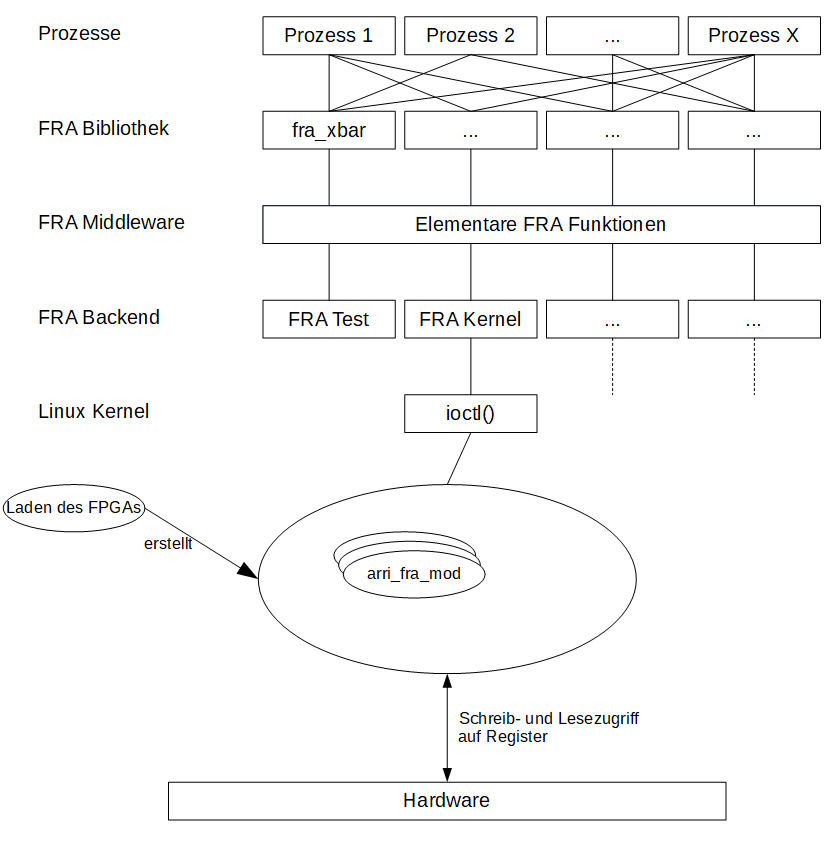
\includegraphics[width = \linewidth]{pictures/2019-11-17_FRA_Overview.png}
	\smallskip
	\caption{Darstellung des Aufbaus des \ac{fra}}
	\label{fig:overview}
\end{figure} 

Die untere Stufe besteht aus verschiedenen backendspezifischen Funktionen. Im folgenden wird nur auf das Kernelbackend eingegangen und das Testbackend wird im Kapitel~\ref{sec:test} erläutert. Im Kernelbackend werden mit den übergebenen Parametern die \ac{ioctl}s (siehe Kapitel~\ref{sec:ioctl}) abgesetzt und somit im Kernel die Hardware gelesen oder beschrieben werden.

%todo glossar middleware
In der \ac{fra} Middleware sind erweiterte Wrapperfunktionen zu finden. Hier werden verschiedene Überprüfungen durchgeführt, damit kein fehlerhafter Zugriff stattfindet. Des Weiteren wird im Wrapper entsprechend dem Backendtyp, die Funktion aus der unteren Ebene ausgewählt. 

Durch die gekapselten Ebenen ist eine Erweiterung um neue Backendtypen einfach gestaltet. 
%Insbesondere über ein Testbackend sollen Unittest zu den verschiedenen Modulen möglich sein, damit können Fehler frühzeitig erkannt, eingegrenzt und behoben werden. 
Aufgrund der Kapselung ist die Wartbarkeit erhöht worden. Dadurch müssen bei Änderungen im Kernelzugriff, nur im Backendcode die entsprechenden Stellen geändert werden.\\

\subsection{\ac{fra} Bibliothek}
Um das \ac{fra} vollständig nutzen zu können, müssen die Geräte geöffnet, geupdatet und auch wieder geschlossen werden. Dies passiert in der sogenannten \ac{fra} Bibliothek. 
Für jeden Modultyp gibt es im \ac{fra} eigene, spezifische Funktionen. Diese Funktionen ersetzen die vorherigen Funktionen, welche direkt in den \ac{fpga} geschrieben haben. Im Rahmen dieser Arbeit wird nur die \ac{xbar} betrachtet und somit auch nur die Implementierung dieser in der Bibliothek.

\begin{lstfloat}
	\begin{lstlisting}
	int32_t fra_xbar(struct fra_handle const *handle, const uint32_t transid, const uint32_t setting)
	{
		int32_t retval = ERRVALUE_SUCCESS;
		uint32_t num, reg;
		
		FRA_CHECK_HANDLE_TYPE(handle, FRA_MOD_TYPE_XBAR);
		
		num = AVALONVIDEO_CROSSBAR_MXN_ENABLE_OUTPUT_REG;
		reg = setting;
		
		retval = fra_set_reg(handle, transid, num, reg);  
		
		return retval;
	}
	\end{lstlisting}
	\captionof{code}{\label{code:fra_xbar} Funktion zum Setzen der \ac{xbar}}
\end{lstfloat}

Für die \ac{xbar} sind fünf spezifische Funktionen implementiert. In diesen Funktionen werden die Einstellungen gesetzt, die aktuellen Registerwerte protokolliert, auf aktuelle Fehlercodes überprüft und der aktuelle Status zurück gegeben. Da in allen Funktionen hauptsächlich auf die \ac{fra} Middleware zugegriffen wird und abgesehen von diesem Zugriff, die Daten aufbereitet werden, wird nur die \textit{fra\_xbar} Funktion exemplarisch betrachtet.\\

In der Funktion im Codeausschnitt~\ref{code:fra_xbar} werden die Ein- und Ausgänge einer \ac{xbar} entsprechend dem übergebenen \textit{setting} verbunden.
Durch das Makro \textit{FRA\_CHECK\_HANDLE\_TYPE} wird überprüft, ob das Gerät im \textit{handle} eine \ac{xbar} ist. Wenn dies nicht der Fall ist, wird ein entsprechender Fehlercode zurückgegeben und die Funktion ist beendet. Diese Überprüfung findet auch bei den restlichen Funktionen in der \ac{fra} Bibliothek statt.
Ist der Modultyp korrekt werden die Übergabeparameter für \textit{fra\_set\_reg} befüllt und die Funktion aufgerufen. Mit dem Zurückgeben des Rückgabewerts der Middleware Funktion ist die Funktion beendet.\\

Finden mehrere Aufrufe in die Middleware statt, wird nach jedem Aufruf der Rückgabewert überprüft und im Fehlerfall direkt die Funktion abgebrochen.


\subsection{\ac{fra} Middleware}
%fra_handle
%Wrapper
%fra_init
%grundfunktionen
Damit die Funktionsaufrufe in der \ac{fra} Bibliothek unabhängig vom Backendtyp funktionieren, werden in der \ac{fra} Middleware Wrapper Funktionen zur Verfügung gestellt. Daneben wird auch eine Struktur zum Verwalten der wichtigen Parameter der \ac{fra} Module im Userspace bereitgestellt.


\begin{lstfloat}
\begin{lstlisting}
struct fra_handle
{
	int dev;
	char dev_type[FRA_MAX_NAME];
	char dev_name[FRA_MAX_NAME];
	uint32_t type_id;
	const struct fra_backend_funcs *backend_funcs;
};
\end{lstlisting}
\captionof{code}{\label{code:fra_handle} Struktur zum Abspeichern wichtiger Parameter}
\end{lstfloat}
Der erste und wichtigste Parameter in der Struktur ist der Dateideskriptor \textit{dev}. Hierüber kann nach dem Öffnen des Geräts weiterhin auf dieses zugegriffen werden. Die restlichen Parameter werden beim Initialisieren des Geräts gesetzt. \textit{dev\_type} und \textit{dev\_name} geben den Modultyp und den Namen an. 
%todo gibt es ersetzen?
Für spätere Überprüfungen gibt es für jeden Modultyp noch eine ID, dieses wird in der Variablen \textit{type\_id} abgelegt. In der \textit{fra\_backend\_funcs} Struktur sind Prototypen aller backendspezifischen Funktionen abgelegt.\\

Das Öffnen eines Geräts ist nur über die \textit{fra\_init} Funktion möglich. Da neben dem Öffnen auch eine Anmeldung bei dem Gerät stattfinden muss (siehe Kapitel~\ref{sec:ioctl}), wird dies über einen Funktionsaufruf abgedeckt. 

In der initialen Funktion \textit{fra\_init} werden verschiedene Einstellungen vorgenommen und Funktionen aufgerufen. Zum einen wird der Funktion ein Backendtyp übergeben und anhand von diesem die Funktionsstruktur im \textit{fra\_handle} gesetzt.
Zum anderen muss neben dem Öffnen des Geräts auch eine Anmeldung vom Prozess stattfinden (siehe Kapitel~\ref{sec:ioctl}). Hierzu werden jeweils die entsprechenden Wrapper Funktionen aufgerufen um die Funktionalität bei allen Backendtypen zu garantieren. Zum Bestimmen von \textit{dev\_type} und \textit{dev\_name} werden auch über eine Wrapper Funktion die Parameter vom Gerät geholt und entsprechend im \textit{fra\_handle} gesetzt. Mithilfe einer Liste, in welcher Name, ID und Größe der einzelnen Module hinterlegt sind, wird die Variable \textit{type\_id} gesetzt. Hierfür wird \textit{dev\_type} mit den Namen der Liste verglichen und bei einem Treffer die entsprechende ID abgespeichert.\\


Die Grundstruktur der Wrapper Funktionen ist für alle identisch, deshalb wird im folgenden beispielhaft die \textit{fra\_set\_reg} näher betrachtet. Grundsätzlich gibt es für jedes konzeptionierte \ac{ioctl} (siehe Kapitel~\ref{sec:ioctl}) im Kernel eine Wrapper Funktion, lediglich für das Logging sind beide \ac{ioctl}s in einer Funktion zusammen gefasst.\\ 


Zu Beginn einer jeden Methode wird über ein Makro verschiedene Überprüfungen durchgeführt. 

\begin{lstfloat}
\begin{lstlisting}
#define FRA_CHECK_HANDLE(p_handle)         \
	if (p_handle == NULL)                    \
	{                                        \
		return ERRVALUE_INVALID_PARAMETER;     \
	}                                        \
	if (p_handle->dev == -1)                 \
	{                                        \
		return ERRVALUE_DEVICE_NOT_OPEN;       \
	}                                        \
	if (p_handle->backend_funcs == NULL)     \
	{                                        \
		return ERRVALUE_NOT_INITIALIZED;       \
	}  
\end{lstlisting}
\captionof{code}{\label{code:fra_check_handle} Makro zum Überprüfen des Handles}
\end{lstfloat}

Ohne ein gültiges Handle würden alle nachfolgenden Aufrufe einen Fehler zurück geben, da alles basierend auf diesem Handle erfolgt. Aus diesem Grund wird in Zeile 2 als Erstes überprüft, ob das \textit{fra\_handle} valid ist. Über den Dateideskriptor kann man herausfinden, ob das Gerät schon geöffnet wurde. Hier wird beim Initiieren der Struktur \textit{dev} auf -1 gesetzt, bei einem geöffneten Gerät ist eine Zahl größer 0 abgespeichert. Als Letztes wird noch überprüft, ob ein Zeiger auf die \textit{fra\_backend\_funcs} Struktur übergeben wurde. Die Funktion, in welcher das Makro aufgerufen wird gibt entsprechende, softwareintern definierte Fehlermeldungen zurück um die Fehlersuche zu erleichtern.\\

In der Funktionssignatur ist immer das \textit{fra\_handle} und die \textit{transid} angeben. Durch das Handle werden alle notwendigen Informationen zum Zugriff auf das Gerät übergeben und die Transaktionsidentifikation \textit{transid} ist in der Signatur implementiert, damit bei einer späteren Erweiterung nicht alle Aufrufe geändert werden müssen. Aktuell wird sie lediglich bis zum Ende durchgereicht und nicht weiter betrachtet, da es kein Teil der Arbeit ist.

\begin{lstfloat}
\begin{lstlisting}
/*  fra_set_reg(handle, transid, num, reg)
 *      sets a register at num
 */
int32_t fra_set_reg(struct fra_handle const *handle,
					const uint32_t transid,
					const uint32_t num, 
					uint32_t reg)
{
	FRA_CHECK_HANDLE(handle);

	if (!handle->backend_funcs->fra_set_reg) return ERRVALUE_FUNCTION_NOT_AVAILABLE;
	return handle->backend_funcs->fra_set_reg(handle, transid, num, reg);
} /* fra_set_reg () */
\end{lstlisting}
\captionof{code}{\label{code:fra_set_reg} Funktion zum Setzen eines Registers}
\end{lstfloat}

Das Makro in Zeile 9 ist im Codeausschnitt~\ref{code:fra_check_handle} näher ausgeführt und im vorhergehenden Absatz genauer erläutert.
Durch die if - Bedingung in Zeile 11 wird überprüft, ob für das ausgewählte Backend die entsprechende Funktion implementiert ist. Ist die Funktion nicht implementiert, liegt an der Stelle ein \textit{NULL} Zeiger. Durch die Überprüfung wird vermieden, dass beim Aufrufen der Funktion auf \textit{NULL} zugegriffen wird und somit beim laufenden Programm ein Fehler auftritt. Der Rückgabewert in der Funktion in der \ac{fra} Middleware entspricht entweder einem entsprechenden Fehlerwert oder dem Rückgabewert der Backendfunktion. 


\subsection{\ac{fra} Kernelbackend}
Da die Wrapper lediglich alle benötigte Übergabeparameter an die Backendfunktionen weiterreichen, haben diese eine identische Funktionssignatur. 
Die einzelnen Funktionen unterscheiden sich im Kernelbackend nur durch die aufgerufenen \ac{ioctl}s und entsprechenden den übergebenden Strukturen dazu. Beispielhaft soll hier wieder die Funktion zum Setzen eines Registers betrachtet werden. \\


Hier finden keine weiteren Überprüfungen statt, da dies bereits eine Ebene höher geschehen ist. Nach dem Füllen der Übergabestruktur wird das \ac{ioctl} aufgerufen und anschließend auf Fehler überprüft. 
Im Fehlerfall wird eine Meldung ausgegeben und der Fehlerwert zurückgegeben. 

\begin{lstfloat}
\begin{lstlisting}
int32_t fra_kernel_set_reg(struct fra_handle const *handle, const uint32_t transid, const uint32_t num, uint32_t reg)
{
	(void) transid;
	int32_t retval = ERRVALUE_SUCCESS;
	int32_t err;
	struct arri_fra_mod_reg frareg;
	
	frareg.num = num;
	frareg.reg = reg;
	err = ioctl(handle->dev, ARRI_FRA_MOD_SET_REG, &frareg);
	if (err < 0)
	{
		error_msg(EH_ERROR, "%s: FRA IOCTL failed. (%u)", handle->dev_name, err);
		retval = ERRVALUE_IOCTL_FAILED;
	}  
	return retval;
} /* fra_kernel_set_reg () */
\end{lstlisting}
\captionof{code}{\label{code:fra_kernel_set_reg} Funktion im Kernelbackend zum Setzen eines Registers}
\end{lstfloat}

\section{Einbindung ins \acl{geo}}\label{sec:soft}
%anlegen der Devices in der software, öffnen der devices über den module_idx und abspeichern im entsprechenden handdle, abändern der funktionen von fpga zugriff auf fra zugriff und hw update lediglich über den module_idx des geo module möglich, da über den identischen namen geöffnet wurde und handle unter dem idx gespeichert ist, umstellen des hw update auf die neuen Funktionen
%Bild?
Um das \ac{fra} vollständig in der Kamerasoftware zum Implementieren müssen die Geräte angelegt, geöffnet, geupdatet und auch wieder geschlossen werden. Dies geschieht an verschiedenen Stellen in der Software und zum Großteil eng verknüpft mit dem \ac{geo}.\\


Angelegt werden die Geräte aktuell beim Laden des \ac{fpga}s. An dieser Stelle ist bekannt, welche Firmware geladen wurde und entsprechend kann über eine Struktur bestimmt werden, ob und an welcher Stelle ein bestimmtes Modul vorhanden ist. Mit einem vorgegebenen Namen und Modultyp werden so die Geräte im Kernel angelegt. Anschließend kann in der kompletten Kamerasoftware davon ausgegangen werden, dass, sofern kein Fehler aufgetreten ist, die Geräte verfügbar sind. Das Anlegen der Geräte soll autark von der Software stattfinden, da dieses in Zukunft ohne die Adressen der Module im \ac{fpga} auskommen soll. Da dieses Konzept den Rahmen der Arbeit übersteigen würde, wird es nicht näher betrachtet. \\

%todo glossar framework
Im \ac{geo} sind die Module der Bildkette in der entsprechenden Reihenfolge abgebildet und über einen Modulindex ist jedes Modul individuell zu unterscheiden. So kann beim initialen Hardwareupdate des \ac{geo} für alle in diesem Framework abgebildeten und vorhandenen Module ein Gerät geöffnet und entsprechend dem Modulindex in ein \textit{fra\_handle} Array abgelegt werden. In beiden Frameworks wird somit über den identischen Modulindex auf das gleiche Modul zugegriffen. Dies spielt vor allem beim Updaten der Module eine wichtige Rolle.


In den Hardwarefunktionen des \ac{geo} werden für die \ac{xbar} die Konfigurationen des Ein- und Ausgänge aus dem Framework abgeholt und anschließend die \textit{fra\_xbar} Funktion (siehe Codeaussschnitt~\ref{code:fra_xbar}) aufgerufen. Analog sollen auch für andere Module die Hardwarefunktionen abgeändert werden.








